
%User Manual
%\chapter{User Manual}
 \chapter{Manual utilizator}

\label{cap:user-manual}
%
%Descrie pașii de instalare și rulare a aplicației. Dacă dezvoltarea aplicației s-a bazat sau a presupus instalarea și configurarea unei infrastructuri (complexe), descrieți detaliat pașii pe care i-ați urmat (referințele utilizate) și mai ales abaterile voite sau necesare de la documenațiile referite. Încercați ca cineva care vă continuă tema să nu mai fie nevoit să mai piardă timp inutil cu pregătirea mediului de lucru și să poată trece cât mai repede la abordarea temei proptriu-zise a proiectului. 
%
%Indincați, de asemenea, explicit versiunile aplicațiilor, bibliotecilor folosite și salvați o copie a acestora pe CD-ul atașat lucrării. E posibil ca aplicația voastră să nu mai funcționeze la fel pe alte versiuni și e bine de știut acest lucru și,  în același timp, e bine ca mediul descris de voi să poată fi reprodus ulterior. 
%
%Se întinde pe aproximativ 2-3 pagini. 

\section{Instalarea proiectului}

Pentru instalarea sistemului, atat timp cat toate dependintele acestuia sunt implinite, utilizatorul nu mai trebuie sa faca nimic. Toate fisierele necesare sistemului au fost impachetate in modulul principal, singurul pas ce poate fi executat de utilizator este crearea unui shortcut catre executabilul ce lanseaza in executie sistemul.
\section{Utilizare}

Dupa deschiderea aplicatiei, utilizatorul este intampinat de meniul de Home al acesteia. In urmatoarea fereastra se poate observa designul acestuia: 

\begin{figure}[h]
	\centering
	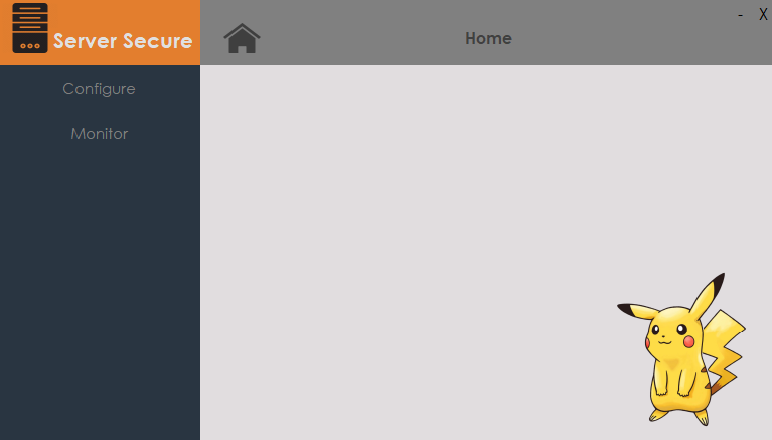
\includegraphics[width=0.6\textwidth]{ui_home.png}
	\caption{Meniul "Home" in interfata grafica}
	\label{fig:ui_home}
\end{figure}

In partea superioara a ferestrei se afla in permanenta numele ferestrei curente(in cazul de fata fereastra Home). In meniul prezent in stanga ferestrei sunt situate celelate doua ferestre disponibile utilizatorului: Configure si Monitor. Utilizatorul poate sa navighze intre aceste ferestre dand un click pe numele ferestrelor, respectiv pe pictograma in forma de casuta pentru meniul Home. \\

\begin{figure}[h]
	\centering
	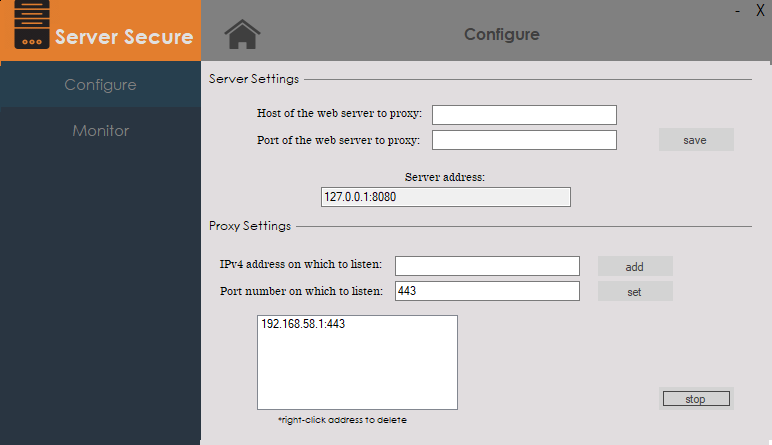
\includegraphics[width=0.7\textwidth]{ui_configure.png}
	\caption{Meniul "Configure" in interfata grafica}
	\label{fig:ui_configure}
\end{figure}

In fereasra Configure, utilizatorul poate sa seteze parametrii de rulare a sistemului. Acestuia i se prezinta doua rubrici: Server Settings si Proxy Settings. In partea de Server Settings, utilizatorul seteaza datele server-ului: adresa IP a acestuia si portul aferent pe care acesta accepta conexiunui. Salavarea sau suprascrierea acestor date se realizeaza prin apasarea butonului "save" din rubrica respectiva. In partea de Proxy Settings, utilizatorul poate sa introduca mai multe adrese IP si un port, pe care sistemul sa accepte conexiuni si sa le redirectioneze catre server. Dupa setarea parametrilor de mai sus, sistemul se poate porni/opri prin apasarea butonului din dreapta jos(cu textul "start"/"stop" dupa caz).
\newpage
\begin{figure}[h]
	\centering
	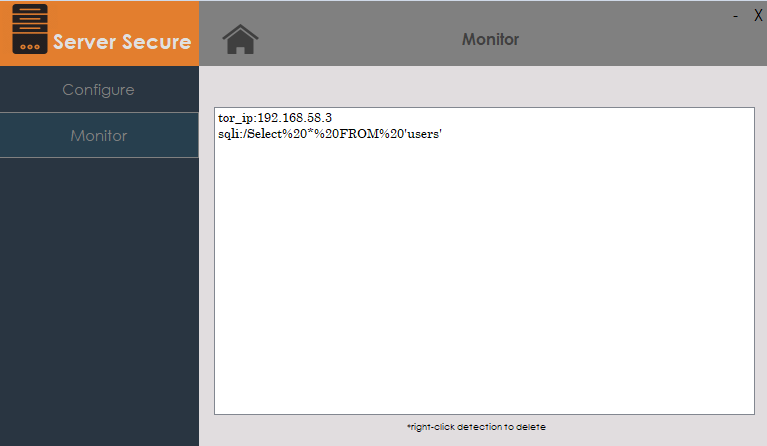
\includegraphics[width=0.8\textwidth]{ui_monitor.png}
	\caption{Meniul "Monitor" in interfata grafica}
	\label{fig:ui_monitor}
\end{figure}

In fereastra de Monitor, utilizatorul poate sa urmareasca activitatea sistemului. In cazul in care sistemul detecteaza un eveniment, acesta este afisat in interfata grafica in aceasta fereastre(conform exemplului din imagine). Daca utilizatorul doreste stergerea evenimentelor antrioare, aceasta se poate realiza prin click dreapta pe eveniment.